\documentclass[12pt]{sismo_iptex}
% IDIOMA
% Se necessário, inserir línguas e indicar língua principal (main)
\usepackage[main=brazil,english]{babel}
\usepackage[italic]{mathastext}
\usepackage{siunitx}
\sisetup{
    group-separator={.},
    group-minimum-digits=3,
    output-decimal-marker={,}}

% Alterando nome do TOC (adicionar em outras línguas, se necessário)
\addto\captionsbrazil{%
	\renewcommand{\contentsname}{SUMÁRIO}
	\renewcommand{\refname}{REFERÊNCIAS}
}
\addto\captionsenglish{%
	\renewcommand{\contentsname}{CONTENTS}
	\renewcommand{\refname}{REFERENCES}
}
% BIBLIOGRAFIA
\usepackage[abnt-emphasize=bf,alf]{abntex2cite}

% Início do documento
\begin{document}

% CAPA 
% Parâmetros
%\docNum{}


%\tipo{BOLETIM SISMOLÓGICO}
%\cancelaDoc{Relatório Técnico nº 123 456-205} % Descomente para opção cancela e substitui
%\cliente{Instituto de Pesquisas Tecnológicas}{IPT}{Av. Professor Almeida Prado, 532}{55555-555}{São Paulo}{SP}

\data{2023}
\titulo{\textbf{RELATÓRIO TÉCNICOS} \\
\unidade{Cidades Infraestruturas e Meio Ambiente}{CIMA}
\lab{Seção de Obras Civis - SOC}
\textbf{Análise dos registros obtidos entre \\}
\periodo{MES/ANO}{MES/ANO}


Cliente
Consórcio empresarial Salto Pilão - CESAP

% Inserir capa
\capa
\pagestyle{timbrado}

% Inserir resumo
%\resumo[]{Teste}{}

%\tableofcontents

\vspace{0.5cm}

%\pagebreak
%\renewcommand{\thepage}{\arabic{page}}
%\setcounter{page}{1}

%\thispagestyle{geral}

\pagestyle{geral}


% Corpo
\pagestyle{tipo_doc}
\setcounter{page}{1}
% Corpo do documento
% INTRODUÇÃO
\section{INTRODUÇÃO}
\par{Este Relatório integra o estudo sismológico em desenvolvimento pelo Consórcio Empresarial Salto Pilão - CESAP e o IPT, de acordo com a Proposta FIPT/IPT n° 59220/21 de 29 de junho de 2021 - “Monitoramento sismológico na área do AHE Salto Pilão, SC, entre julho/2021 e junho/2024”, em continuidade aos trabalhos iniciados em janeiro de 2007 (Carta Proposta CT-Obras/SG-233/06), referentes à implantação do programa de monitoramento da sismicidade induzida na Usina Hidrelétrica Salto Pilão - UHESP. O estudo visa o atendimento aos requisitos do Projeto Básico Ambiental - PBA deste empreendimento, em execução na bacia do rio Itajaí-Açu, nos municípios de Lontras, Ibirama e Apiúna, no Estado de Santa Catarina, dentro do Programa 3: Monitoramento dos Impactos Geológicos – Sub-Programa 3.2: Sismicidade Induzida, de acordo com a LAO – Licença Ambiental de Operação no 4.055/12 concedida pela Fundação do Meio Ambiente - FATMA do Estado de Santa Catarina, atualmente Instituto de Meio Ambiente de Santa Catarina - IMA.}

\subsection{Objetivo}
\par{O objetivo deste trabalho é apresentar os resultados do monitoramento sismológico efetuado na área da Usina Hidrelétrica Salto Pilão, com a Estação Sismológica SP7, entre 01 de dezembro de 2022 e 30 de junho de 2023, permitindo acompanhar a sismicidade local e orientar a adoção de eventuais medidas mitigadoras, atendendo às exigências previstas no processo de licenciamento ambiental do empreendimento.}


% ATIVIDADES EXECUTADAS E RESULTADOS OBTIDOS
\section{ATIVIDADES REALIZADAS E RESULTADOS OBTIDOS}
\par{O método de análise utilizado baseia-se nas técnicas atualmente empregadas pela Sismologia, desenvolvidas para a análise dos dados obtidos por meio de estação sismológica digital triaxial, com a utilização de softwares específicos.}

\par{Os resultados das análises dos dados registrados foram dispostos em figuras e tabelas que constam nos Apêndices A e B, respectivamente, para melhor apresentação e facilidade de leitura do texto deste Relatório.}

\subsection{Características operacionais}
\label{subsec:caracteristicas}
\par{Os dados foram obtidos por meio da Estação SP7, composta dos seguintes equipamentos:}
\begin{itemize}
    \item Digitalizador (DAS – Data Acquisition Sub-system), modelo 130-01 (RefTek, EUA), de alta resolução, com 3 canais de registro, 24 bits, número de série 9FD3;
    \item Sistema interno de gravação (DRS – Data Recording Sub-system) em flash cards (SimpleTech, EUA), capacidade de 2 GB (com 4 unidades, sendo duas instaladas na estação e, as outras duas, para troca na coleta de dados);
    \item Relógio GPS (RefTek);
    \item Sismômetro, modelo SeisMonitor (Oyo GeoSpace, EUA), número de série 1430;
    \item Painel solar, modelo SQ75-P de 75W/12Vcc, com controlador de carga BaseD (Artesa, Espanha), números de série 028222A1180544787 e 02090579, respectivamente;
    \item Bateria, estacionária, selada, 12 Vcc e 100 Ah (Freedom, DF2000);
    \item Palmtop, modelo MEL1000 (Meazura-Acceca, Austrália), utilizado para processar o software de operação dos equipamentos sismológicos. \\
A operação da estação é realizada por meio do software PFC-130 (Palm Field Controller), que é o controlador de ajuste de campo para o DAS130, versão palmtop. Com este software, são fornecidos, entre outros, os parâmetros de operação dos equipamentos, verificado o funcionamento da estação e transferidos os dados; e
    \item Multiteste, modelo ET1610 (Minipa, Brasil).
\end{itemize}

\par{Para transferência dos dados de campo para a sede do IPT, em São Paulo, foi utilizada a leitora de flash cards, modelo FlashLink (SimpleTech, EUA), número de série STI-UMC2300 e para arquivamento, um PC de uso geral do CESAP.}
\par{As coletas dos dados foram efetuadas por técnicos da UHSP, mediante troca dos flash cards. O encaminhamento dos dados para o IPT ocorreu a partir do envio dos mesmos na plataforma OneDrive para posterior processamento e análise.}
\par{A rotina de coleta e análise dos dados foi mantida. O Palmtop que serve para controle dos equipamentos da estação apresentou problemas de conexão na coleta do dia 14.06.2021, e consequentemente perdeu o arquivo de configurações da estação SP7 na memória. Após tentativas infrutíferas de restaurar a conexão com a estação, o Palmtop foi enviado ao IPT para reconfiguração, e foi consertado e enviado de volta à estação SP7, que resumiu sua operação normal no dia 01.09.2021. Desde então a estação opera normalmente. Entretanto, para o período entre 15.06.2021 e 01.09.2021 não houve registro de dados, e consequentemente desmontes/eventos sísmicos que pudessem ter ocorrido durante esse período não foram detectados. Desde então, a estação operou de modo satisfatório, sem que houvesse perdas de dados que comprometessem as análises.}
\par{Uma planilha de campo, contendo a sequência de tarefas que devem ser executadas a cada coleta de dados ou visita à estação, foi preenchida com informações que permitiram a avaliação do desempenho dos equipamentos instalados na estação sismológica. Além destas informações operacionais, foram anotados os problemas observados e toda atividade desenvolvida durante os trabalhos de campo. No Anexo A estão apresentadas as planilhas de campo.}
\par{O IPT realizou visita de campo à estação SP7 no dia 21.06.2022, para inspeção geral da estação sismológica e para instalação do novo equipamento GPS adquirido. A estação se encontra em bom estado de conservação, e o equipamento novo foi instalado sem grandes dificuldades, funcionando de imediato com o DAS em operação no local e adquirindo lock com a constelação de satélites em poucos segundos. Foi também averiguado que a provável fonte do ruído que se observa na estação de maneira intermitente em período comercial vem de uma bomba de água que se encontra instalada a aproximadamente 15 metros da estação. A estação opera de maneira satisfatória na maior parte do tempo, não comprometendo o monitoramento sismológico da área, e, portanto, este ruído intermitente é tolerável.}
\par{Além da verificação das informações contidas na planilha de campo e nos arquivos de gerenciamento do sistema, o técnico que está realizando a análise dos dados sismológicos faz uma interpretação das características dos sinais sísmicos para verificar se não está ocorrendo alguma anormalidade.}
\par{No dia 12.12.2007, às 19 h e 11 min (hora universal), iniciou-se a operação da Estação Sismológica SP7 situada nas coordenadas geográficas: 27,1203º S (6.999.291 UTM-N), 49,4620º W (652.443 UTM-E) e cota de 489 m (esta localização foi apresentada com detalhe no Desenho 1 do Relatório IPT no 98 859-205 – “Definição e instalação da estação sismológica na área do Aproveitamento Hidrelétrico Salto Pilão, SC”, emitido em fevereiro de 2008.}
\par{O sismômetro foi instalado e orientado de acordo com os pontos cardeais, de modo que os canais 1, 2 e 3 de registro correspondessem, respectivamente, às componentes Z (vertical), NS (Norte-Sul) e EW (Leste-Oeste). Vale observar que o cabo de ligação digitalizador-sismômetro veio montado com as polaridades das componentes horizontais invertidas. Devido à montagem deste cabo não foi possível inverter as ligações dos pinos destas componentes. Assim, foi decidido que, no IPT, quando processados os dados de campo, a inversão de polaridade seria realizada por meio do software de análise.}
\par{Na instalação da Estação SP7, foram utilizados os flash cards identificados com os números 1 e 2. Na primeira coleta de dados, estes flash cards foram substituídos pelos de números 3 e 4. Nas coletas seguintes, continuou-se a substituição, utilizando estes pares de flash cards de modo alternado.}
\par{O funcionamento da Estação SP7 pode ser visualizado, de modo geral, na Figura 1, Apêndice A. Nesta figura apresenta-se o gráfico de completeza mensal, mostrando a disponibilidade dos dados da estação SP7 no período de referência deste relatório. Em síntese, no período de monitoramento sismológico compreendido entre 01.12.2022 e 30.06.2023, o funcionamento da Estação SP7 pôde ser considerado satisfatório. Um detalhamento maior do funcionamento da estação para o período englobado por este relatório pode ser obtido analisando-se os boletins sísmicos no Anexo A, que contêm os gráficos de completeza diários para cada mês entre 01.12.2022 e 30.06.2023.}

\subsection{Interpretação dos registros}
\label{subsec:interpret}
\par{Este item abrange a interpretação de cada evento identificado, localizado e quantificado.}
\par{Para a determinação da distância epicentral, o azimute e a magnitude dos eventos registrados na Estação SP7, adotou-se a metodologia apresentada no Relatório IPT no 104 490-205 – “Análise dos registros obtidos entre 12 de dezembro de 2007 e 29 de maio de 2008, na Estação Sismológica SP7, SC”, emitido em julho de 2008.}

\subsubsection{Detonações em pedreiras e obras}
\par{O conhecimento e o controle do cronograma de detonações em pedreiras e obras situadas próximas à área do empreendimento são de grande importância na interpretação dos registros e análise dos dados, pois facilitam a identificação dos eventos associados às detonações.}
\par{O controle, de um modo geral, é efetuado por meio de planilhas, nas quais são declarados os dias e horários dos fogos, cargas, tipo de fogo e outras informações referentes às detonações efetuadas, que são periodicamente (geralmente mensalmente) enviadas ao IPT por mensagem eletrônica.}
\par{Na área do entorno do empreendimento foram identificadas duas pedreiras em funcionamento (pedreiras Azza e Daclande) e vários pontos com atividades minerárias que podem utilizar explosivos no processo de lavra. Destaca-se que no Desenho 1 do Relatório IPT no 98 859‑205 foram apresentadas as localizações destas pedreiras e minerações.}
\par{Neste período de análise foram recebidas informações sobre detonações das pedreiras Azza e Daclande para os meses de dezembro de 2022 e janeiro, fevereiro, março, abril, maio e junho de 2023. Com os dados das detonações realizadas procurou-se identificá-las nos registros dos eventos obtidos instrumentalmente. Os eventos foram classificados como detonações suspeitas ou sismos a partir da análise da forma de onda do registro sísmico e do horário de ocorrência, junto à inspeção via satélite pelo software Google Earth Pro, para averiguar a presença de operações de mineração nas proximidades dos epicentros determinados.}
\par{Foi identificado um total de sessenta e sete (67) desmontes/detonações no período, sendo sete (7) destes confirmados através do plano de fogo provido pelas pedreiras (Daclande e Azza), e outros doze (12) localizados nas imediações das mesmas, as quais foram relacionadas a detonações não informadas por estas pedreiras devido à localização dos epicentros, às características dos sinais sísmicos e aos horários de ocorrência semelhantes aos das detonações que já vinham ocorrendo nestes locais. Já os outros quarenta e oito (48) eventos registrados não puderam ser correlacionados com os dados recebidos das pedreiras conhecidas, mas pela característica do sinal sísmico, horário de ocorrência e pela verificação de que existem empreendimentos de mineração/pedreiras não identificadas na região, foram classificados como tal.}
\par{Ressalta-se que todos os registros classificados como detonações (com ou sem confirmação) apresentaram magnitude pequena, condizente com diferentes tipos de detonações nestes empreendimentos, sendo as magnitudes mínima e máxima registradas de 0.4 e 3.0 MLv, respectivamente.}
\par{A Tabela 1, Apêndice B, contém a relação dos eventos que foram associados às detonações, incluindo a data e o horário de registro (em hora universal), o epicentro, magnitude e energia liberada, além de um comentário indicando a pedreira associada, quando o epicentro localizado consta no plano de fogo. A Figura 2, Apêndice A, mostra a localização em volta do empreendimento para as detonações identificadas no período.}
\par{Como as informações advindas de detonações sempre serão úteis na interpretação dos dados, solicita-se que, periodicamente, seja verificada a existência de novas pedreiras/obras na área, obtidas as suas respectivas localizações e efetuados os contatos com os responsáveis, com o intuito de se obter os correspondentes “planos de fogo”.}

\subsubsection{Sismos naturais}
\par{No período de 01.12.2022 a 30.06.2023, foram detectados três pequenos sismos locais próximos à estação SP7, com magnitudes entre 0.2 e 0.9 MLv. O maior destes eventos foi registrado em 2023-05-26 18:31:02 (UTC). Suas localizações com relação à estação SP7 são mostradas na Figura 2, Apêndice A.}
\par{Foi detectado um sismo regional natural no território brasileiro, na região do Vale do Ribeira, no estado de São Paulo, próximo à cidade de Iguape – SP, em 2023-06-16 11:22:00 (UTC). O sismo teve magnitude 4.0 mR, e foi sentido por diversas pessoas na região e também em áreas distantes do epicentro, como na capital paulista. O registro do evento na estação SP7 é mostrado na Figura 3, Apêndice A. O registro pela estação teve excelente qualidade e auxiliou a determinação do mecanismo focal (determinação de orientação da falha) do evento em conjunto com as estações da Rede Sismográfica Brasileira.}
\par{Não foram detectados telessismos no território brasileiro durante o período. Os telessismos fora do Brasil e imediações, embora registrados, não foram avaliados neste estudo que visa caracterizar a sismicidade ocorrida na área da Usina Salto Pilão. Os epicentros localizados no Brasil são localizados para contribuir com o melhor conhecimento da sismicidade nacional.}
\par{Continuam válidas as considerações e orientações anteriores a respeito das medidas a serem tomadas em caso de ocorrência de um sismo local sentido pela população.}
\par{Para o período de 01.12.2022 a 30.06.2023 foram emitidos os Boletins Sísmicos nos 18/36-2024 a 24/36-2024, apresentados no Anexo A.}

\subsubsection{Sismos induzidos}
\par{O monitoramento da sismicidade induzida por reservatório na área de influência do Empreendimento da Usina Hidrelétrica Salto Pilão, que está na fase do pós-enchimento, não indicou a existência de eventos relacionados à operação deste reservatório.}
\par{Porém, recomenda-se que a auscultação sismológica na região seja mantida, de modo a dar continuidade ao melhor conhecimento da sismicidade local e regional, além do necessário acompanhamento da operação da UHE Salto Pilão.}



% QUADRO SISMOTECTÔNICO
\section{QUADRO SISMOTECTÔNICO}
\par{Os aspectos sismotectônicos da área da Usina Hidrelétrica Salto Pilão foram discutidos no Relatório IPT no 98 859-205, emitido em fevereiro de 2008.}


% CONSIDERAÇÕES FINAIS
\section{CONSIDERAÇÕES FINAIS}
\label{sec:consid_finais}

\par{Para o monitoramento sismológico realizado no período de 01.12.2022 a 30.06.2023, tem-se que:}

\begin{itemize}
    \item Em síntese, o funcionamento da Estação SP7 pôde ser considerado satisfatório. Um detalhamento maior do funcionamento da estação para o período englobado por este relatório pode ser obtido analisando-se os boletins sísmicos no Anexo A, que contêm os gráficos de completeza diários para cada mês no período.
    \item Na área de influência do empreendimento foram registrados sessenta e sete (67) desmontes com magnitudes entre 0.4 e 3.0 (MLv), sendo quatorze (19) destes relacionados a detonações nas proximidades das pedreiras Azza e Daclande, e os restantes em outras áreas (Figura 2, Apêndice A).
    \item Foram detectados três pequenos sismos locais próximos à estação SP7, com magnitudes entre 0.2 e 0.9 MLv. O maior destes pequenos eventos foi registrado em 2023-05-26 18:31:02 (UTC).
    \item Foi detectado um sismo regional natural no território brasileiro, próximo à cidade de Iguape – SP, em 2023-06-16 11:22:00 (UTC). O sismo teve magnitude 4.0 mR .
    \item Durante o monitoramento sismológico local efetuado com a Estação SP7 não foram registrados sismos induzidos oriundos da operação do reservatório. 
    \item A orientação e procedimentos apresentados no Relatório IPT no 115 463-205 – “Análise dos registros obtidos entre 1º de junho e 30 de novembro de 2009, na Estação Sismológica SP7, SC”, emitido em janeiro de 2010, e no Relatório IPT no 120 081-205 – “Análise dos registros obtidos entre 1º de junho e 30 de novembro de 2010 na Estação Sismológica SP7, Salto Pilão, SC e síntese das atividades e dos resultados do monitoramento sismológico”, emitido em janeiro de 2011, quanto à ocorrência de provável tremor de terra sentido pela população local ou ocorrências anômalas na área do empreendimento, devem ser mantidos.
\end{itemize}

\par{O monitoramento instrumental possibilita determinar o epicentro, quantificar o tamanho (a magnitude), definir a origem do evento e, se for o caso, em função da análise do comportamento espaço-temporal da atividade, tomar medidas mitigatórias.} 
\par{Assim, pelos resultados do monitoramento sismológico realizado com a Estação SP7, em função das características operacionais do registrador-sismômetro e de sua localização, considera-se de muita valia manter esta estação em funcionamento para dar continuidade no conhecimento da sismicidade local e regional.}
\par{No monitoramento realizado não foi observada a ocorrência de evento sísmico associado à implementação do Empreendimento da UHE Salto Pilão. A continuidade do monitoramento sismológico na área do empreendimento permitirá acompanhar eventual ocorrência local.}
\par{Mantidas as atuais características da sismicidade, local e regional, para a continuidade do monitoramento sismológico devem ser mantidos os atuais procedimentos adotados para operação, coleta e análise dos dados, com periodicidade mensal. Além disso, continuam válidas as orientações a serem adotadas no caso de ocorrer evento local sentido pela população e de eventuais anomalias na obra tais como desplacamentos de rochas e estampidos associados.}

\assinaturaDoisDigitalRelatorio


% EQUIPE TÉCNICA
\section{EQUIPE TÉCNICA}
\label{sec{equip_tec}

\par{\textbf{IPT}}
\par{\textbf{UNIDADE DE NEGÓCIOS CIDADES, INFRAESTRUTURA E MEIO AMBIENTE}}
\par{\textbf{Seção de Obras Civis}}
\par{Lucas Alexandre Schirbel – Me., Físico, Astrônomo, – FIPT.}
\par{Emília Maria dos Santos Brasílio – Meteorologista, Técnica – FIPT.}
\par{\textbf{Apoio Administrativo}}
\par{Ludmila Souto Lima Parisi – Secretária – FIPT.}
\par{Silmara Frari Landim – Técnica Administrativa.}
\par{\textbf{USINA HIDRELÉTRICA SALTO PILÃO}}
\par{Pedro Nogueira de Oliveira – Analista de Meio Ambiente}


\clearpage
\newpage


% Bibliografia
\section{REFERÊNCIAS BIBLIOGRÁFICAS}
%\renewcommand{\refname}{REFERÊNCIAS}
%\addcontentsline{toc}{section}{REFERÊNCIAS}
\bibliography{ref}

% APENDICE A
\clearpage
\vspace*{\fill}
\section*{\centering APÊNDICE A \\ FIGURAS}
\vspace*{\fill}
\clearpage
\newpage


% COMPLETUDE

\begin{figure}[ht!]
    \centering
 	\captionsetup{justification=justified, singlelinecheck=false, width=1\textwidth}
    \caption{Gráfico de completeza mensal para os dados da estação SP7. O detalhamento diário da completeza para cada mês pode ser averiguado nos boletins sísmicos mensais no Anexo A.}
    \begin{mdframed}[
        linecolor=black,
        linewidth=1pt,
        roundcorner=10pt,
    ]
    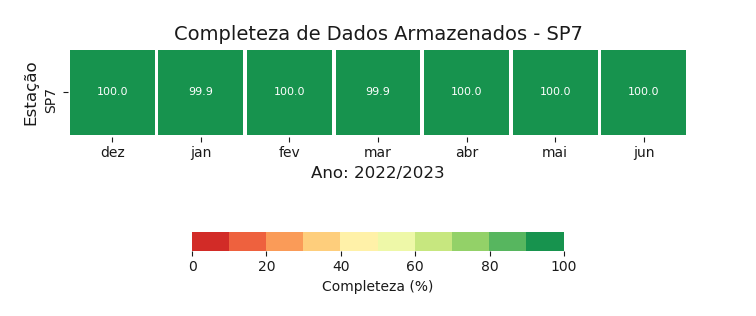
\includegraphics[width=1.0\textwidth]{./relatorio/figuras/completude.png}
    \end{mdframed}
    \caption*{Fonte: IPT}
\end{figure}

\newpage
% MAPA 

\begin{figure}[ht!]
	\captionsetup{justification=justified, singlelinecheck=false, width=1\textwidth}
    \caption{Mapa do entorno do empreendimento mostrando pontos de interesse e os epicentros dos eventos classificados como detonações e sismos. Foram detectados um total de sessenta e sete (67) eventos associados a detonações no período, classificados a partir do horário de ocorrência e da forma de onda, além do plano de fogo fornecido, com magnitudes mínima e máxima de 0.4 e 3.0 MLv, respectivamente.}
    \begin{mdframed}[
        linecolor=black,
        linewidth=1pt,
        roundcorner=10pt,
    ]
    \begin{center}
    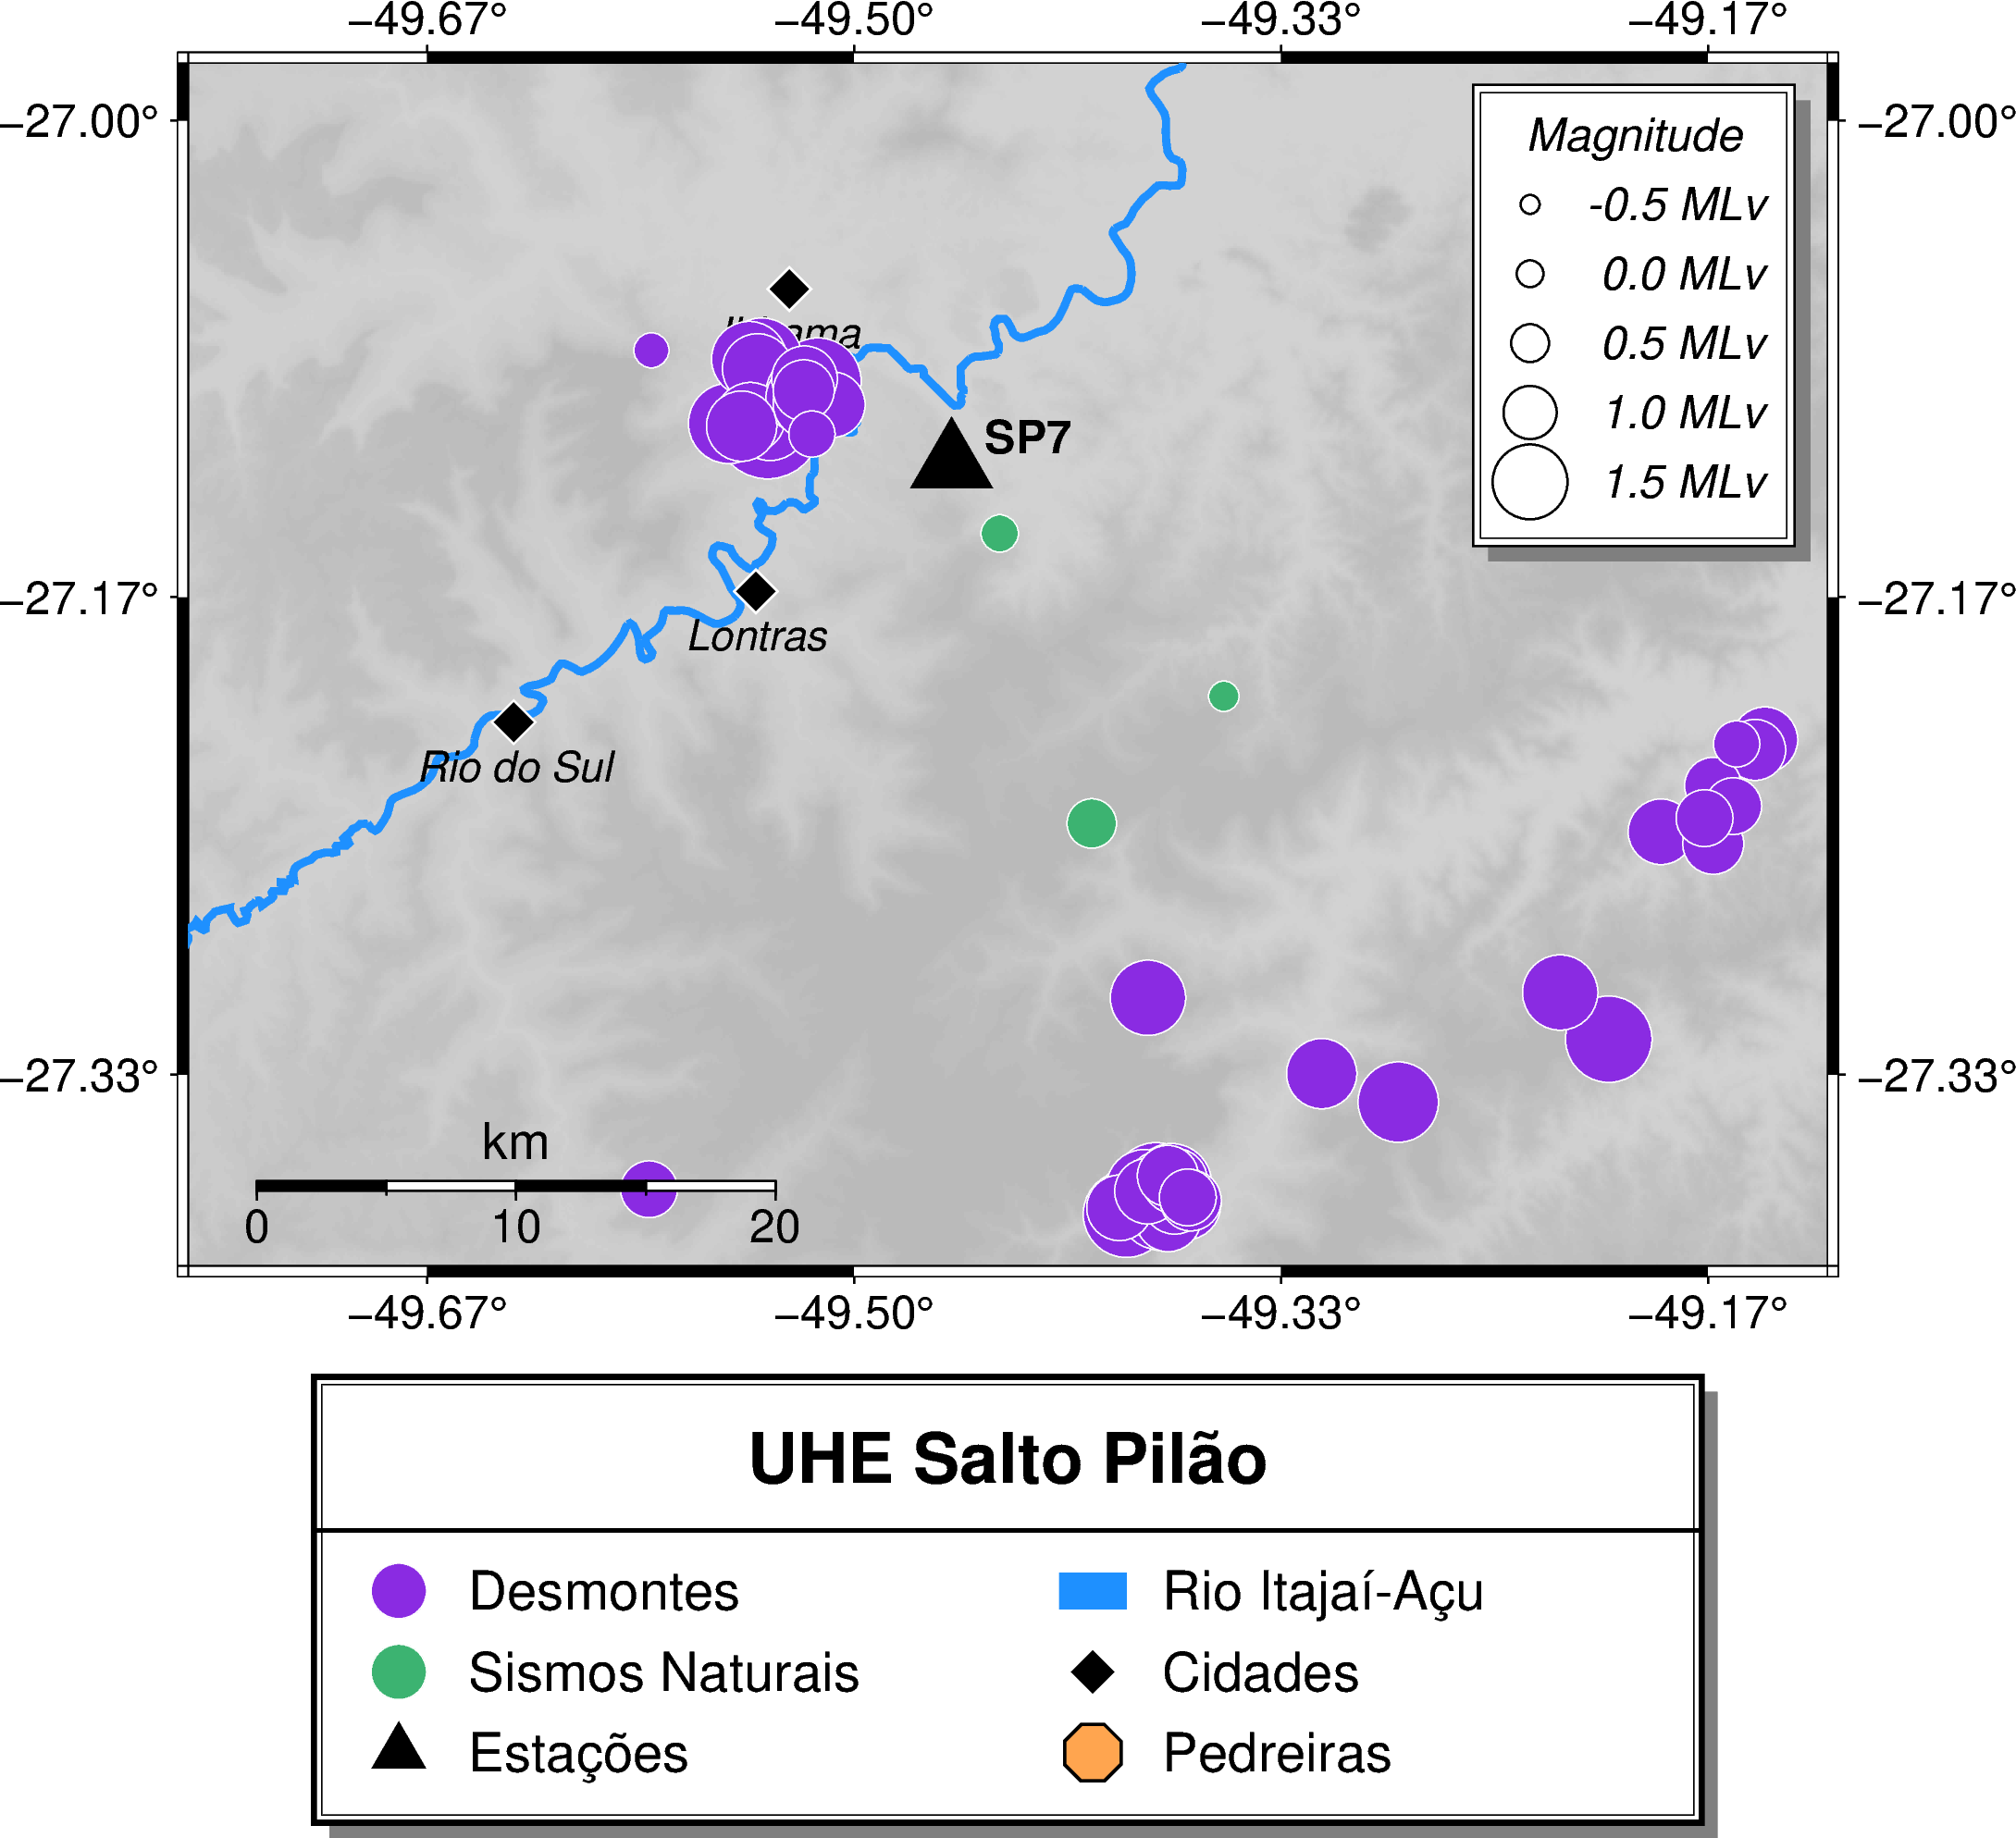
\includegraphics[width=0.8\textwidth]{./relatorio/figuras/mapa.png}
    \end{center}
    \end{mdframed}
    \caption*{Fonte: IPT}
\end{figure}

\newpage
% REGIONAL 

\begin{figure}[ht!]
	\captionsetup{justification=justified, singlelinecheck=false, width=1\textwidth}
    \caption{Evento regional natural registrado em 2023-16-06 11:22:00 (UTC) nas proximidades da cidade de Iguape – SP. A) Localização do evento (círculo vermelho maior) em relação à estação SP7 (círculo vermelho menor) e B) Forma de onda do evento registrada na estação SP7.}

    \begin{mdframed}[
        linecolor=black,
        linewidth=1pt,
        roundcorner=10pt,
    ]
    \textbf{A}
    \begin{center}
    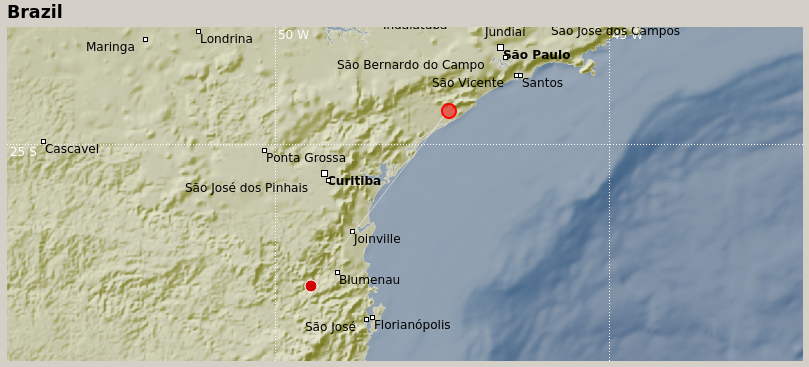
\includegraphics[width=0.8\textwidth]{./relatorio/figuras/regiao.png}
    \end{center}
    \end{mdframed}
    \begin{mdframed}[
        linecolor=black,
        linewidth=1pt,
        roundcorner=10pt,
    ]
    \textbf{B}
    \begin{center}
    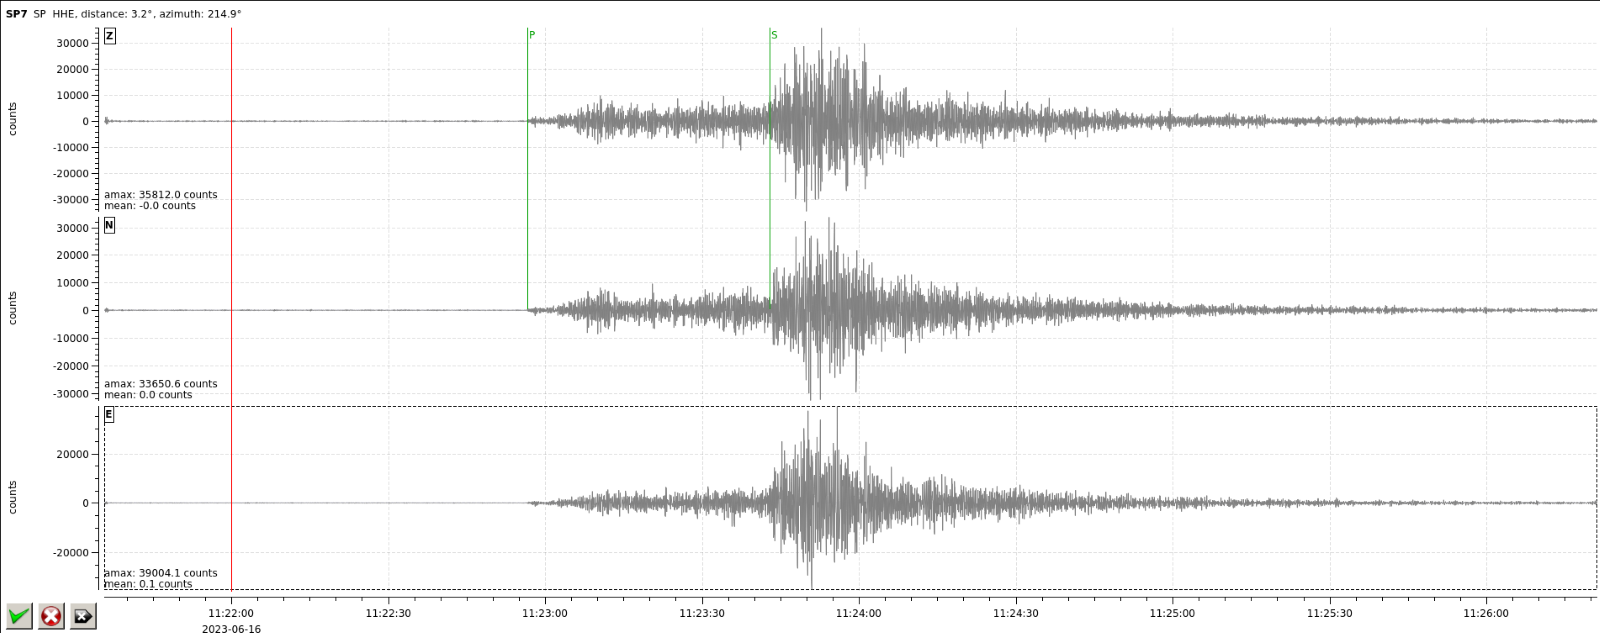
\includegraphics[width=0.8\textwidth]{./relatorio/figuras/evento_regional.png}
    \end{center}
    \end{mdframed}

    \caption*{Fonte: IPT}
\end{figure}



% APENDICE B
\clearpage
\vspace*{\fill}
\begin{center}
    \section*{APÊNDICE B}
    \textbf{TABELAS}
\end{center}
\vspace*{\fill}
\clearpage
\newpage


\begin{center}
\scriptsize
\setlength{\arrayrulewidth}{0.05pt}
\begin{longtable}{ccccS[table-format=6.0]S[table-format=7.0]ccc}
\captionsetup{justification=justified,singlelinecheck=false}
\caption{Listagem de eventos detectados e categorizados durante o período de interesse.\\ A coluna \textit{Cat} representaria a categoria na qual o evento foi classificado sendo \textit{Q}=Detonação/Desmontes, \textit{E}=Sismo Regional e \textit{I}=Sismo induzido e \textit{N}=Não-localizável. O valor da energia para os sismos foi obtido a partir da magnitude através da relação proposta por Richter (1958).}\\
%%%%%%%%%%%%%%%%%%%%%%%%%%%%%%%%%%%%%%%%%%%%%%%%%%%%%%%
\hline \\[-4ex]
\hline \\[-5ex]
\multicolumn{1}{c}{ID} &
\multicolumn{1}{c}{Hora de Origem (UTC)} &
\multicolumn{1}{c}{Longitude} &
\multicolumn{1}{c}{Latitude} &
\multicolumn{1}{c}{UTM X} &
\multicolumn{1}{c}{UTM Y} &
\multicolumn{1}{c}{MLv} &
\multicolumn{1}{c}{Energia} &
\multicolumn{1}{c}{Cat} \\


\\[-5.0ex] \hline
\\[-5.0ex]

\multicolumn{1}{c}{\textit{{}}} & 
\multicolumn{1}{c}{\textit{{}}} & 
\multicolumn{1}{c}{\textit{(\textdegree\hspace{0.25em})}} & 
\multicolumn{1}{c}{\textit{(\textdegree\hspace{0.25em})}} & 
\multicolumn{1}{c}{\textit{{(m)}}} & 
\multicolumn{1}{c}{\textit{{(m)}}} & 
\multicolumn{1}{c}{\textit{{}}} & 
\multicolumn{1}{c}{\textit{{(J)}}} & 
\multicolumn{1}{c}{\textit{{}}} \\ 

\\[-5.0ex] \hline
\\[-4.0ex]
\endfirsthead


%%%%%%%%%%%%%%%%%%%%%%%%%%%%%%%%%%%%%%%%%%%%%%%%%%%%%%%
\hline \\[-4ex]
\hline \\[-5ex]
\multicolumn{1}{c}{ID} &
\multicolumn{1}{c}{Hora de Origem (UTC)} &
\multicolumn{1}{c}{Longitude} &
\multicolumn{1}{c}{Latitude} &
\multicolumn{1}{c}{UTM X} &
\multicolumn{1}{c}{UTM Y} &
\multicolumn{1}{c}{MLv} &
\multicolumn{1}{c}{Energia} &
\multicolumn{1}{c}{Cat} \\


\\[-5.0ex] \hline
\\[-5.0ex]

\multicolumn{1}{c}{\textit{{}}} & 
\multicolumn{1}{c}{\textit{{}}} & 
\multicolumn{1}{c}{\textit{(\textdegree\hspace{0.25em})}} & 
\multicolumn{1}{c}{\textit{(\textdegree\hspace{0.25em})}} & 
\multicolumn{1}{c}{\textit{{(m)}}} & 
\multicolumn{1}{c}{\textit{{(m)}}} & 
\multicolumn{1}{c}{\textit{{}}} & 
\multicolumn{1}{c}{\textit{{(J)}}} & 
\multicolumn{1}{c}{\textit{{}}} \\

\\[-5.0ex] \hline
\\[-4.0ex]
\endhead
\hline
\caption*{Fonte: IPT.}

\endlastfoot
%%%%%%%%%%%%%%%%%%%%%%%%%%%%%%%%%%%%%%%%%%%%%%%%%%%%%%%
MC\_20230830\_183917 & 2023-08-30T18:39:17 & -49,7253 & -27,1233 & 626336 & 6999266 & 1,3 & \num[round-precision=3,round-mode=figures,scientific-notation=true]{192765} & Q \\
MC\_20230824\_152934 & 2023-08-24T15:29:34 & -49,8028 & -27,1492 & 618629 & 6996476 & 1,5 & \num[round-precision=3,round-mode=figures,scientific-notation=true]{489398} & Q \\
MC\_20230822\_153204 & 2023-08-22T15:32:04 & -49,8803 & -26,8769 & 611218 & 7026705 & 1,7 & \num[round-precision=3,round-mode=figures,scientific-notation=true]{1.40658e+06} & Q \\
MC\_20230818\_154804 & 2023-08-18T15:48:04 & -49,7430 & -27,2696 & 624424 & 6983077 & 1,5 & \num[round-precision=3,round-mode=figures,scientific-notation=true]{665616} & Q \\
MC\_20230815\_192736 & 2023-08-15T19:27:36 & -49,8482 & -27,9594 & 613296 & 6906757 & 1,2 & \num[round-precision=3,round-mode=figures,scientific-notation=true]{150265} & Q \\
MC\_20230815\_191541 & 2023-08-15T19:15:41 & -50,5589 & -27,8340 & 543432 & 6921103 & 1,5 & \num[round-precision=3,round-mode=figures,scientific-notation=true]{620197} & E \\
MC\_20230815\_152902 & 2023-08-15T15:29:02 & -49,7932 & -27,1799 & 619550 & 6993060 & 1,8 & \num[round-precision=3,round-mode=figures,scientific-notation=true]{2.4461e+06} & Q \\
MC\_20230814\_152826 & 2023-08-14T15:28:26 & -49,8405 & -27,0239 & 615021 & 7010383 & 1,1 & \num[round-precision=3,round-mode=figures,scientific-notation=true]{86207.8} & Q \\
MC\_20230809\_105318 & 2023-08-09T10:53:18 & -51,3027 & -27,6952 & 470149 & 6936521 & -0,9 & \num[round-precision=3,round-mode=figures,scientific-notation=true]{14.7546} & I \\
MC\_20230808\_180349 & 2023-08-08T18:03:49 & -51,6466 & -27,3376 & 436040 & 6976001 & 0,5 & \num[round-precision=3,round-mode=figures,scientific-notation=true]{7229.98} & Q \\
MC\_20230808\_124749 & 2023-08-08T12:47:49 & -51,9186 & -28,7091 & 410272 & 6823898 & 1,3 & \num[round-precision=3,round-mode=figures,scientific-notation=true]{201872} & Q \\
MC\_20230803\_180211 & 2023-08-03T18:02:11 & -52,0653 & -28,7992 & 396036 & 6813799 & 1,5 & \num[round-precision=3,round-mode=figures,scientific-notation=true]{541480} & Q \\
MC\_20230802\_202746 & 2023-08-02T20:27:46 & -50,5841 & -27,9327 & 540915 & 6910184 & 1,4 & \num[round-precision=3,round-mode=figures,scientific-notation=true]{335748} & Q \\
MC\_20230802\_154527 & 2023-08-02T15:45:27 & -51,2518 & -27,4233 & 475109 & 6966653 & 0,8 & \num[round-precision=3,round-mode=figures,scientific-notation=true]{24333.2} & Q \\
MC\_20230801\_182340 & 2023-08-01T18:23:40 & -49,6500 & -27,1915 & 633720 & 6991634 & 1,2 & \num[round-precision=3,round-mode=figures,scientific-notation=true]{142694} & Q \\
MC\_20230801\_181715 & 2023-08-01T18:17:15 & -49,6761 & -27,6211 & 630624 & 6944073 & 1,9 & \num[round-precision=3,round-mode=figures,scientific-notation=true]{3.50567e+06} & Q \\
\end{longtable}
\end{center}
\clearpage



% ANEXOS 
\clearpage
\vspace*{\fill}
\begin{center}
    \section*{ANEXO A}
    \textbf{DOCUMENTOS GERAIS} \\
    \textbf{(ART, Planilhas de campo e Boletins Sísmicos)}
\end{center}
\vspace*{\fill}
\clearpage
\newpage

\input{}


\end{document}
